\chapter{Architecture Exploration}\label{models}
This chapter presents the proposed neural network architectures. It starts with a baseline TNN network implemented in \texttt{PyTorch}, which then undergoes a series of hardware-aware adaptions specific to jet tagging. During this process two separate architectures are developed, which differ by the input type and design goal. The first one, referred to as the \textit{ultra-low latency} one, targets the HLF jet representation and aims to achieve the lowest possible latency at the cost of accuracy and AUC values. The second one, called \textit{accuracy-focused}, is based on the constituent list jet representation and trade-offs latency for quality of classification while still remaining within L1T timing constraints. In the end, the mechanism of quantization-aware training is explained, with a proposed way of implementing it in this project.


\section{Base Architecture}
The starting point of this analysis is derived from transformer architecture used in the original paper \cite{44-vaswani2017attention} and recent proof-of-concept used for jet tagging \cite{3-yuan2021constituentnet:}. The overview of the network components can be seen in figure \ref{fig:constituent-net}.

\begin{figure}[hpt!]
  \centering
  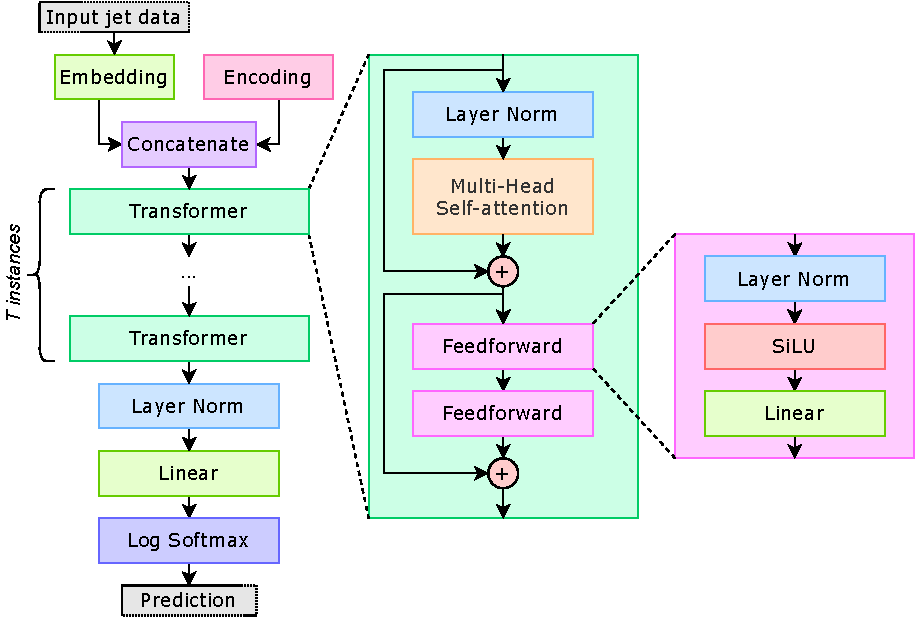
\includegraphics[trim={0cm 0cm 0cm 0cm}, width=0.6\textwidth, center]{models/constituent_net.pdf}
  \caption{Diagram with an overview of the baseline architecture.}
  \label{fig:constituent-net}
\end{figure}

The straight-forward path between model's input and output highlights the sequential nature of transformer which stands in opposition to recurrency present in GRU and LSTM models. While this allows for the aforementioned parallelizability and pipelining on FPGAs, it also poses a challenge of increased hardware footprint and synthesis complexity when compared to recurrent models, where the key components can get reused to meet the resource constraints. To better understand the transformer's complexity, the next subsections derive the equations linking the internal components and explain the involved terminology.


\subsection{Input embedding and Residual Connections}
Although the model lacks any recurrency, the transformer includes two residual connections which have been widely adopted since their successful application in ResNet neural networks \cite{75-kaiming2016deep}. They offer improvements to training time and resulting accuracy \cite{74-szegedy2016inception-v4}, however, they require standardized data dimensionality to ensure the summation can be logically executed. In this project, this is obtained thanks to input embedding, which transforms the input \(\bm{\hat{x^i}} \in \mathbb{R}^{L \times 16} \) into a shape \(\mathbb{R}^{L \times d}\) that is used through the design, as seen in equation \ref{eq:embedding}. The \(d\) size is referred to as the self-attention latent or embedded dimension.

\begin{equation}\label{eq:embedding}
  \bm{\hat{x^i}_{\text{emb}}} = \text{embedding} ( \bm{\hat{x^i}} ) = w_{\text{embed}}\; \bm{\hat{x^i}} + b_{\text{embed}} \in \mathbb{R}^{L \times d}
\end{equation}

This dimensionality change can be conveniently performed using a linear layer, and it has to be remembered that each such layer increased the model learning capacity thanks to the learnable weights and bias. The network's inner dimension \(d\) is treated as a hyperparameter as it influences the model's accuracy and performance, but it has to be noted that the other dimension prevalent in the network comes from the input's number of jet constituents \(L\) (which is set to 1 in case of the HLS representation), meaning that the model is also susceptible to a parameter which cannot be easily tuned.


\subsection{Input Encoding}
Along the embedding, an input encoding is concatenated and fed to the transformer layer. In natural language processing, the encoding is meant to allow the model to benefit from the sequential information of the words in a sentence. It can be obtained from a sinusoidal function using the position index or simply treated as another learnable parameter. The sequential relations are not present in the jet data, because all the jets originate from the same proton-proton collision, hence, the latter approach is used in this project. It is worth mentioning, that from empirical analysis, the learnable encodings have a significant impact on the final results as they represent a trained, hidden state concatenated to all inputs during evaluation, as shown in equation \ref{eq:encoding}. Its impact is especially prevalent for the HLF data (where \(L = 1\)), where the hidden state matched input's dimension and effectively doubles it after concatenation.

\begin{equation}\label{eq:encoding}
  \text{encoding} ( \bm{\hat{x^i}_{\text{emb}}} ) = w_{\text{encoding}} \in \mathbb{R}^{1 \times d} \implies \text{concat} (\bm{\hat{x^i}_{\text{emb}}},\; w_{\text{encoding}}) \in \mathbb{R}^{(L+1) \times d}
\end{equation}

Choosing a learned hidden state is also more efficient for inference in hardware, as the increased training cost associated with back-propagation of this parameter yields a constant set of values that are known during compile-time of the FPGA and can be implemented using a LUT.


\subsection{Normalization and Parameter Extraction}
As layer normalization does not track and gather running mean and variance statistics, this mechanism is implemented on top of the existing \texttt{PyTorch} implementation to facilitate extracting the aggregated statistics after training. These, along with all the learned weights and biases, are extracted and transformed into specific C++ formats supported in HLS using a custom tool developed for this purpose. This allows for directly initializing the FPGA's BRAMs and LUTs with the model parameters, which avoids the need for an interaction with a host machine.

Obtaining the statistics taken for the data before normalization layers can also be viewed as a hardware-aware optimization. This can be explained with the mathematical derivation presented in equation \ref{eq:normalization-optimization}

\begin{equation}\label{eq:normalization-optimization}
  y = \frac{x - E[x]}{\sqrt{Var[x] + \epsilon}} \cdot \gamma + \beta = x \cdot (\frac{\gamma}{\sqrt{Var + \epsilon}}) + (\beta - \frac{\gamma * E}{\sqrt{Var + \epsilon}}) = w \cdot x + b
\end{equation}

By treating the mean \(E[x]\) and variance \(Var[x]\) of input \(x\) as learned parameters, the square root and division operations can be fully omitted by fusing them into the existing \(\gamma\) and \(\beta\) parameters which simplifies the hardware required for the normalization layers. This is especially useful as FPGAs lack dedicated hardware for these computationally expensive operations, which could lead to suboptimal designs being synthesized. Independently of the implementation in this work, a similar idea has been proposed and successfully used as an optimization in the past \cite{46-fan2018real-time}.

The algorithm behind the parameter extraction is rather simple, and the difficulty comes from the domain specific knowledge of handling \texttt{PyTorch} model parameters and generating the correct files for HLS. The break-down of the necessary steps can be seen in algorithm \ref{alg:parameter-extraction}.

\begin{algorithm}
  \caption{Mechanism behind model parameter extraction}\label{alg:parameter-extraction}
  \begin{algorithmic}[1]
    \State $state \gets $load\_state(model)
    \State sort($state$)
    \State $curr\_weight \gets $null
    \For{$param$ in $state$}
      \State $mean \gets $find\_mean(model, param)
      \State $var \gets $find\_var(model, param)

      \If{$param$ is weight}
        \State $curr\_weight \gets $param
        \State $new\_param \gets $update\_weight(param, var)

      \Else
        
        \State $new\_param \gets $update\_bias(param, curr\_weight, mean, var)
      \EndIf
      \State \texttt{save(new\_param)}
    \EndFor
  \end{algorithmic}
\end{algorithm}



\section{Ultra-Low Latency Architecture}
The first of the proposed architectures targets the HLF representation dataset, where each sample is of \(\mathbb{R}^{1 \times 16}\) dimensions, making it a better candidate for an \(N\) times faster inference than the constituent list representation with inputs with \(\mathbb{R}^{N \times 16}\) dimensions. The simpler data means that the network can achieve satisfactory classification results with a lower learning capacity, hence allowing for various simplifications of the base architecture.

\subsection{Optimization and Tuning}
The hypothesis leading the optimization process is that the HLF dataset can be learned by a relatively lower complexity network. The strategy is to start with the accuracy and AUC value of the base architecture and keep applying changes to the network as long as they do lead to significant drops in classification results, with detailed evaluation discussed in 
\cref{evaluation}. Doing so is inherently beneficial for the later FPGA mapping, as even without hardware-aware changes, a simpler model is likely to require fewer resources and achieve lower latency.

The architecture features that have the highest influence on the overall performance are the size of the latent dimension and number of transformer layer. In the case of the original transformer model \cite{44-vaswani2017attention}, 12 transformer layers are used, split equally into a decoder and encoder parts of the networks. This, along with latent dimension size of 512 shows that jet tagging requires significantly less complexity compared to natural language processing, as the recent ConstituentNet \cite{3-yuan2021constituentnet:} is based on only 3 transformer layers and embedded dimension of 64. However, as the latter network targets a more complex dataset, the first optimization performed in this project yielded a reduction to only a single transformer layer with latent size of 16. The network complexity is directly proportional to the number of layers, while the self-attention complexities shown in \cref{self-attention} can be simplified given the dimensions of \textit{queries}, \textit{keys}, and \textit{values} are shared and equal to \(\in \mathbb{R}^{N \times d}\) in this work, 
as shown in equation \ref{eq:qkv-complexity-time-simple} and \ref{eq:qkv-complexity-space-simple} for time and space respectively. It is worth mentioning that the shared dimension \(d\) is purposefully represented this way as it is equal to the model embedded dimension \(d\).

\begin{equation}\label{eq:qkv-complexity-time-simple}
  \mathcal{O}(h \cdot (N_Q N_K (d_Q + d_V) + d_Q^2 (N_Q + N_K) + d_V^2 N_K + N_Q d_V d_{out}) )) \equiv
  \mathcal{O}(h N d (N + d + d_{out}) ))
\end{equation}

\begin{equation}\label{eq:qkv-complexity-space-simple}
  \mathcal{O}(h \cdot (N_Q (N_K + d_V) + d_Q (N_Q + N_K) + d_V N_K + N_Q d_{out}) )) \equiv
  \mathcal{O}(h N (N + d + d_{out}) ))
\end{equation}

Another successful optimization was simplifying the SiLU to ReLU activations, as in hardware, the latter rely on a single comparator to determine whether to pass input to output directly or set the signal to zero. In contrary, SiLU requires computing the sigmoid function as well as performing a multiplication, which has a non-trivial cost on an FPGA.

Interestingly, the layer normalization was first changed to batch normalization to simplify the tracking and embedding the running data statistics. This only leads to a marginal accuracy decrease, however, it is interesting to point out that so does removing the normalization layers from the design. This can be attributed to the "smoother" distribution of elements of the normalized HLF dataset, which tend to average around zero instead of taking values from a wide range as it is the case for the constituent list representation, shown in figure TODO. Hence, the used dataset does not benefit from additional normalization, vastly simplifying the architecture.

\todofig{Simple visualization of the distribution in HLF and constituent list}
\todofig{|}
\todofig{|}
\todofig{|}
\todofig{|}

\subsection{Summary}
The optimizations described in the previous subsection correspond to a noticeably simpler architecture, which can be seen in figure \ref{fig:constituent-net-simplified}. It is also worth mentioning that the simplifications targeted the components of the transformer block other than the multi-head self-attention block. This is a result of the used mechanism's key role in the learning process as well as the fact that it is difficult to modify it as it uses very basic components, and changing them would impact the underlying, commonly-approved function.

\begin{figure}[hpt!]
  \centering
  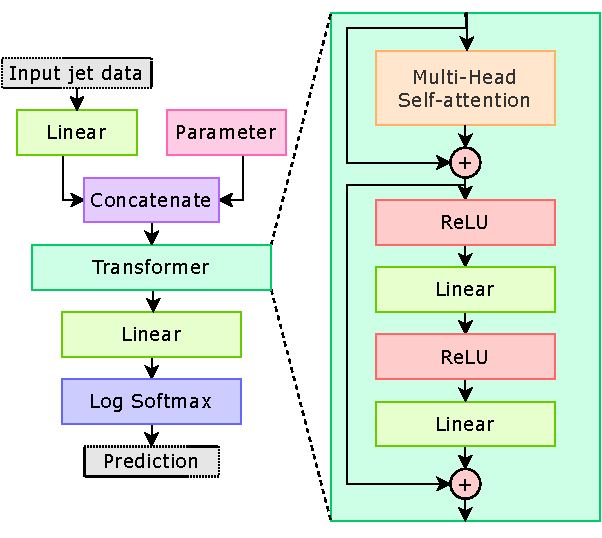
\includegraphics[trim={0cm 0cm 0cm 0cm}, width=0.45\textwidth, center]{models/constituent_net_simplified.pdf}
  \caption{Diagram with an overview of the ultra-low latency architecture.}
  \label{fig:constituent-net-simplified}
\end{figure}


\section{Accuracy-Focused Architecture}\label{accuracy-focused-model}
The aim of the second architecture is to exploit a bigger design along with the more complex constituent list dataset to achieve a higher accuracy and AUC value that the ultra-low latency model while still meeting the latency constraints of L1T at LHC. In addition, this design undergoes a design space exploration to compare and reason about a number of existing and novel techniques.

\subsection{Optimization and Tuning}
Aside from the increase in computational complexity, the biggest difference caused by changing the datasets is the vastly different range and distribution of samples, showcased in figure TODO. While the network could perform normalization as its first layer, this approach was tested to significantly degrade the results quality. This is likely due to the fact that each samples' feature follows a distinct distribution and lays within a different range, so normalizing causes a loss in the carried information. These distributions can be seen in figure TODO. \maybe{Maybe claim visual differences between distributions of HLF and constituent list}

Normalization and data distribution also need to be discussed for a different reason in the context of this architecture. The layer normalization layers present in the base design are not completely omitted this time, and instead changed to batch normalization. Although the layer normalization characteristic of not tracking running statistics and relying on per-layer normalization during evaluation can yield improvement to classification results, it is not a desired behavior for FPGA mapping due to the lack of hardware support for the square root and division operations. This could be resolved in an analogous way to batch norm by simply manually tracking the statistics, but this was experimentally proven to substantially affect the accuracy. What is more, the less clustered and more diverse distributions of constituent list dataset features lead to numerical instability in softmax calculations of the exponential function. Even though this was a marginal issue for the PyTorch implementation, it was quickly observed to drastically change the expected outcome of the early HLS prototype implementations. A solution to this issue lays in using additional normalization layers just before the self-attention softmax blocks, which not only solved this problem, but also very slightly increased the learning capacity of the network.

\begin{figure}[hpt!]
  \centering
  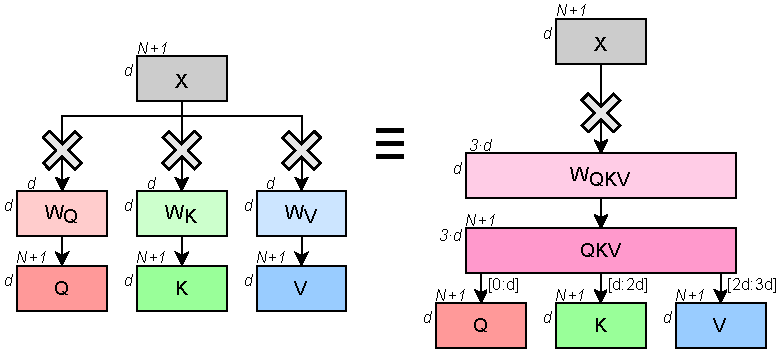
\includegraphics[trim={0cm 0cm 0cm 0cm}, width=0.7\textwidth, center]{models/weight_merging.pdf}
  \caption{Simple illustration for equivalency between matrix multiplication using merged and unmerged weights on the example of \textit{queries}, \textit{keys}, and \textit{values} used in self-attention.}
  \label{fig:weight-merging}
\end{figure}

It is a common for GPU training to merge together adequately shaped fully-connected layers, as seen in figure \ref{fig:weight-merging}. This allows the GPU to more optimally use its resources for the computation, potentially decreasing the training time without affecting the results. Nonetheless, this approach was dropped for this architecture to avoid generating one bigger weight matrix in favor of several smaller ones. Contrary to GPUs, the synthesis process for FPGAs benefits from smaller precomputed matrices as it is easier for the algorithm the map them to certain BRAMs or LUTs that are close to the components that read from or write to them. With the significantly smaller dimension sizes for the ultra-low latency model, this aspect generated negligible difference, while in this architecture the merged weight matrix size would exceed a reasonable size and lead to an extremely long synthesis process and likely suboptimal hardware mapping.

Lastly, some optimizations are inherited from the ultra-low latency architecture. The SiLU are replaced by ReLU activations, while embedding and encoding are simply implemented by a fully-connected layer and a learnable parameter. When it comes to the transformer layer count and latent dimension size, they follow the configuration of ConstituentNet of 3 and 64, however, a closer evaluation and discussion about these are carried in \cref{evaluation}.

\subsection{Summary}
In this case, the resulting architecture is much more similar to the base one in terms of its overall structure, however it differs from it with the crucial changes to normalization layers, activation function and modifications to the multi-head self-attention block. The overview of this design can be seen in figure \ref{fig:constituent-net-accuracy}.

\begin{figure}[hpt!]
  \centering
  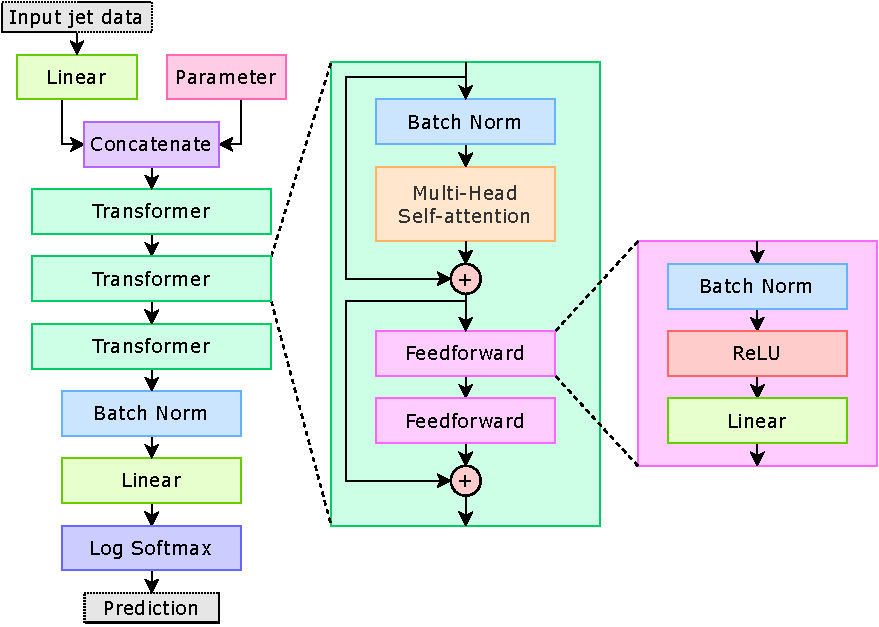
\includegraphics[trim={0cm 0cm 0cm 0cm}, width=0.6\textwidth, center]{models/constituent_net_accuracy.pdf}
  \caption{Diagram with an overview of the accuracy-focused architecture; the inclusion of batch normalization before softmax within the multi-head self-attention block is not showcased for the sake of clarity.}
  \label{fig:constituent-net-accuracy}
\end{figure}


\section{Quantization-Aware Training}\label{pre-training-quantization}
The use of the term \textit{quantization} in the topic of machine learning and reconfigurable hardware might appear as a misnomer if one follows the definition used in signal processing, where it refers to constraining continuous values to a set of discrete ones. However, this definition can be extended for converting values from a very large set of discrete values to a 
significantly smaller ones. This is the case when half (16 bits), single (32 bits) or double (64 bits) precision floating-point numbers are expressed using a fixed-point representation. This leads to an inherent quantization noise because many distinct values in floating-point representation map to the same number when stored as fixed-point, which can be seen in figure \ref{fig:float-to-fixed} \cite{76-shaumontfixed}. Although this work exploits fixed-point arithmetic for its efficient hardware representation, it has to be noted that quantizing is also used for time and space efficient GPU inference as it can vastly lower the total bits used across model's weights, hence reducing the required memory and computational complexity.

\begin{figure}[hpt!]
  \centering
  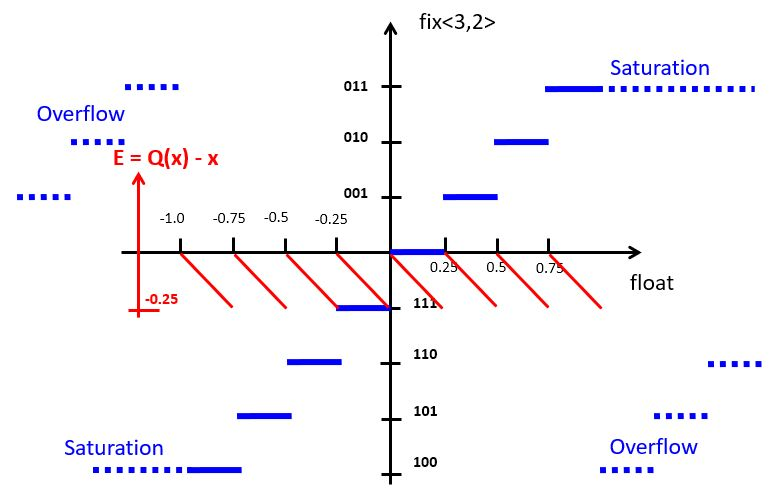
\includegraphics[trim={0cm 0cm 0cm 0cm}, width=0.6\textwidth, center]{models/float_to_fixed.jpg}
  \caption{Quantization noise from 32-bit floating-point to 3-bit (2-bit integer, 1-bit fractional) fixed-point representation; widths selected to highlight the behavior. Two methods of handling values outside representable range are showed: classic overflow as well as saturation to minimum or maximum value.}
  \label{fig:float-to-fixed}
\end{figure}

\subsection{Floating-point and Fixed-point Representations}
To bring more perspective to this topic, let's start by observing the 16-bit wide floating-point notation with an example seen in equation \ref{eq:floating-point}. \textit{SIGN}, \textit{EXP} and \textit{FRAC} stand for the sign, exponent and fractional\footnote{Also referred to as \textit{significand precision}} fields (sequences of 1's and 0's) of a number.

\begin{equation}\label{eq:floating-point}
  \{\text{SIGN | EXP | FRAC}\} = 
  \begin{cases}
    (-1)^{\text{SIGN}} \cdot 2^{-14} \cdot (0.\text{FRAC}_2) & \text{EXP} = 00\_000_2 \\
    (-1)^{\text{SIGN}} \cdot 2^{\text{EXP}-15} \cdot (1.\text{FRAC}_2) & \text{EXP} \in [00\_000_2,\; 11\_110_2] \\
    \pm \infty & \text{EXP} = 11\_111_2
  \end{cases}
\end{equation}

The widths of the fields for standard floating-point width can be seen in table \ref{tab:floating-point-widths}, however, the particular details in the example do not need to be fully understood to notice the required complexity of the hardware design to perform operations using floating-point values. It has to first decode each of the fields, check for special values, normalize inputs to a common base, perform the computation, and lastly normalize again and decode the fields. As it can be expected, this comes with a significant overhead compared to integer numbers.

\begin{table}[hpt!]
  \centering
  \caption{Comparison of standard precision types for floating-point values. Note the difference in half precisions, where \textit{Brain} offers same the exponent width as single precision, and \textit{binary} priorities fractional precision.}
  \label{tab:floating-point-widths}
  \begin{tabular}{|c|c|ccc|}
  \hline
  \multirow{2}{*}{\textbf{Precision}} & \multirow{2}{*}{\textbf{Total width}} & \multicolumn{3}{c|}{\textbf{Field width}}                                    \\ \cline{3-5} 
                                      &                                       & \multicolumn{1}{c|}{sign} & \multicolumn{1}{c|}{exponent} & fractional \\ \hline
  \textbf{Double}                     & 64                                    & \multicolumn{1}{c|}{1}    & \multicolumn{1}{c|}{11}       & 52         \\ \hline
  \textbf{Single}                     & 32                                    & \multicolumn{1}{c|}{1}    & \multicolumn{1}{c|}{8}        & 23         \\ \hline
  \textbf{Half} (\textit{Brain})               & 16                                    & \multicolumn{1}{c|}{1}    & \multicolumn{1}{c|}{8}        & 7          \\ \hline
  \textbf{Half} \textit{(binary})              & 16                                    & \multicolumn{1}{c|}{1}    & \multicolumn{1}{c|}{5}        & 10         \\ \hline
  \end{tabular}
\end{table}

While dedicated circuits exits in CPUs and GPUs to accelerate floating-point calculations, FPGAs tend to use fixed-point representation to achieve superior latency with relatively simple hardware resources. It comprises a sequence of \textit{P} binary digits representing the integer part, then a virtual decimal point, followed by \textit{R} binary digits representing the fractional part, according to equation \ref{eq:fixed-point}.

\begin{equation}\label{eq:fixed-point}
  \{ I_{P-1} | ... | I_0 | F_{R-1} | ... | F_0 \} = I_{P-1} \cdot 2^{P-1} + ... + I_{0} \cdot 2^{0} + F_{R-1} \cdot 2^{-1} + ... + F_{0} \cdot 2^{-R}
\end{equation}

The virtual decimal point is not explicitly present in the number, instead the lengths of the sequences are stored which allows for correct handling. There are also no widely adopted standards for the internal widths of fixed-point numbers, as they are often implementation-specific. Fixed-point hardware is only responsible for correctly aligning the inputs in case they vary in width, which is an information know at compile-time, as opposed to run-time for floating-point numbers, which makes it very suitable for FPGAs.

\subsection{Existing Implementations}
Quantization-aware training refers to training a model using the fixed-point representation of numbers to allow the model to reduce the impact of the quantization noise by learning the underlying data characteristics with less precision. However, approaches differ in the degree to which the quantization is used as it can be applied to training data, weights and biases, intermediate results or any combination of these. It also has to be noted that existing implementations have been designed with different objectives, although to the best of our knowledge, the most widely used ones are still in their very experimental phases at the time of writing this report. The approaches considered for this work are listed below:

\begin{itemize}
  \item \textbf{PyTorch Eager Mode Quantization} \cite{77-krishnamoorthistatic} - currently in a \textit{beta} version. PyTorch offers two development modes - Eager, for research purposes and easier experimentation, as well as Script, for production use cases \cite{79-sharmapytorch}. This quantization scheme is an extension to the former mode and requires manual handling of the placement of quantizing and dequantizing layers in a network as well as operator fusion and functional blocks. Currently, offers no support for the vanilla recurrent block, LSTM, GRU or self-attention.

  \item \textbf{PyTorch FX Graph Mode Quantization} \cite{78-zhangfx} - similarly to the previous point, it is in a \textit{prototype} version, and it extends the graph-base and speed-focused Script mode. This leads to an easier implementation as the quantization feature support process happens automatically. It does not work for convolutional, self-attention or embedding layers yet.

  \item \textbf{Brevitas} \cite{brevitas} - a research project from a team at Xilinx, a major reconfigurable hardware vendor. It is early in its development cycle, but it promises to support most network architectures, provided that all existing layers are replaced with their quantized variants, and quantizing and dequantizing is also handled manually, similarly to PyTorch Eager Mode Quantization. Its caveat is that while it provides a granular, per-variable level of bit-width customization, the offered fixed-point widths cannot be easily changed in size.

  \item \textbf{QPyTorch} \cite{zhang2019qpytorch} - a Cornell University research project, which offers a fixed-point simulation framework. Existing networks can be easily adapted to it, only requiring manual quantization layers usage throughout the design. These can be of arbitrary width, which supports a rich design space exploration, however, the representation of widths, biases, accumulators and gradients needs to follow the same quantization scheme for all layers, which is dictated my the training optimizer configuration.
\end{itemize}

It is clear that each described solution comes with its own advantages and disadvantages. Even though the first two approaches come officially from PyTorch, they lack support for the core transformer layer - the self-attention. Hence, this report proposes the latter two for research on quantized transformer architectures and their hardware implementations.

\begin{figure}[hpt!]
  \centering
  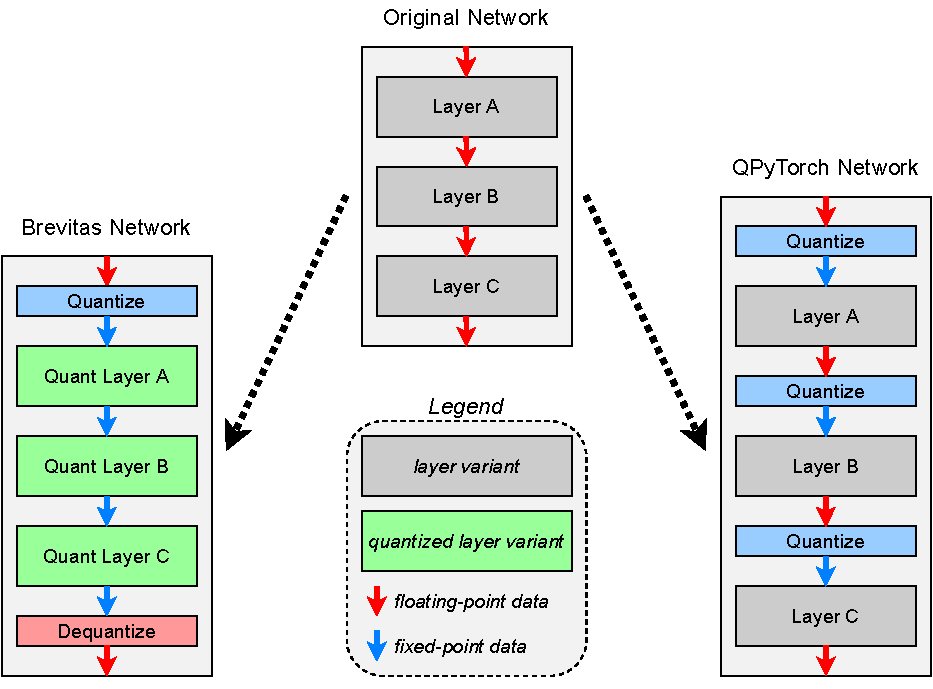
\includegraphics[trim={0cm 0cm 0cm 0cm}, width=0.7\textwidth, center]{models/pre-training-quantization.pdf}
  \caption{Comparison of a simple neural network prepared for quantization-aware training using Brevitas and QPyTorch frameworks.}
  \label{fig:pre-training-quantization}
\end{figure}

Figure \ref{fig:pre-training-quantization} showcases the designs resulting from quantizing a simple neural network using Brevitas and QPyTorch. The former approach relies on library-provided quantized variants of commonly found neural layers, and each can have its input's, output's and internal parameters' bit-width configured separately to one of the pre-defined types. This technique is more truthful to how FPGAs operate, but at the same time, more demanding in terms of implementation complexity than QPyTorch's one, which exploits the wide range of PyTorch's native layers and only requires custom quantizing blocks in between them. The latter is also slightly less computationally intensive, however both methods results in significantly longer training time than the floating-point representation due to the lack of support for fine-tuned, fixed-point GPU implementation of the network layers. It is also worth mentioning, that Brevitas offers a convenient way of exporting the quantized models to Xilinx hardware representations as well as external tool chains. Lastly, quantization is also proposed and discussed as a post-training mechanism in \cref{post-training-quantization}, with both approaches then evaluated and compared in \cref{evaluation}.
